% arara: lualatex
% !TEX TS-program = LuaLaTeX

\documentclass{coderdojo}

\worksheet{2}{Take Away}

\begin{document}

\maketitle

\section*{Introduction}

In this worksheet we will create a version of the Take Away game:
\begin{exercise}
Game consists of a pile of coins with two players taking turns to play. At each turn the player decides to take 1, 2 or 3 coins.  The player who take the last coin wins.

\centerline {\includegraphics[page=12]{take_away_game}}
\end{exercise}

We will build a number of versions of this game --- each version gets better and more complicated! You can choose what type of improvements/extensions you find more interesting. I don't expect that we will get all versions completed.

\begin{dingautolist}{192}
\item \hyperref[sec:basic]{\color{section}\bfseries Basic game}

We start by implementing the basic game where the computer is pretty stupid and only takes one coin each time.

\item \hyperref[sec:StopHumans]{\color{section}\bfseries Stop humans cheating!}

A big issue when writing programs that interact with people is that we cheat! Or to put it more nicely, we humans, don't always follow instructions as well as we should.  So we need to write code to check that the human player's input is valid. 

\item \hyperref[sec:GoRandom]{\color{section}\bfseries If can't get smarter then go random}

Currently our computer player is pretty stupid (it always takes one coin).  There is no challenge here. We want it to be better than that. In the next version we will make it better, but in this version we will --- using just one line of code --- make it {\bfseries appear} much smarter by adding randomness. 

\item \hyperref[sec:GetSmarter]{\color{section}\bfseries Get smarter}

In this version we will make the computer smarter --- this is often called artificial intelligence --- by enabling it to make decisions on how many coins to take based on the number of coins remaining in the game.

\end{dingautolist}

At this point we could go in many different directions:
\begin{itemize}
\item
We could look at variations of the game. For example, we could change the rules regarding how many coins we are allowed to remove. To make this really hard we could have gaps, such as you are allowed to take 1, 3, or 4 coins but not allowed to take 2.
\item
Or we could go graphical --- this will be the focus of next handout.
\end{itemize}

%%\item \hyperref[sec:Fancy]{\color{section}\bfseries Fancier input and output}
%
%All of the input and output  so far has been in the prompt panel (called Shell) at the bottom of the screen. We can do better!
%
%%\item \hyperref[sec:GoGraphical]{\color{section}\bfseries Go graphical}
%
%In our final version (if we ever get here!) is the write a graphical version of the game using python's turtle library.



\section{Basic game}\label{sec:basic}

We start by implementing the basic game where the computer is pretty stupid and only takes one coin each time. The main 
items to note here are:

\begin{itemize}
\item[\color{section!70!black}\larger\ding{43}] A game will have three stages:
\begin{enumerate}
\item Setup game
\item Play game
\item Report result at end of game.  
\end{enumerate}
So to start, open a new file using menu {\bfseries File$\to$New} and enter the following comments

%%\pythonexternal{code/TakeAway_Start.py}
%\centerline{\begin{minipage}{.9\textwidth}
%\ACODE{2}{6}{code}{TakeAway_Start.py}{filename=false}{}
%\end{minipage}}

\codeonly{}{2}{6}{code}{TakeAway_Start.py}

Save this script as \code{TakeAway_Basic.py}. Right now the script does nothing! Comments are only there to help us.
%\begin{tcblisting}{title=boo}
%\end{tcblisting}

\item[\color{section!70!black}\larger\ding{43}] In the setup (initialisation) stage we will need create a variable to store the number of coins left in the game. And to make the game more interesting/difficult we want to start with a random number of coins, say between 15 and 25 coins. So we import the python module \code{random}. This module contains functions for generating random numbers.

%\centerline{\begin{minipage}{.9\textwidth}
%\ACODE{3}{3}{code}{TakeAway_Basic.py}{filename=false}{}
%\end{minipage}}

\codeonly{}{3}{3}{code}{TakeAway_Basic.py}
	
Then we generate a random integer\footnote{An {\bf integer} is a whole number.}and store it in a variable, \code{coins}, for later using

%\centerline{\begin{minipage}{.9\textwidth}
%\ACODE{4}{4}{code}{TakeAway_Basic.py}{filename=false}{}
%\end{minipage}}

\codeonly{}{4}{4}{code}{TakeAway_Basic.py}

Next, we need some way of recording whose is next to move. To use this we use another variable, \code{isComputerMove}, as follows
	
%\centerline{\begin{minipage}{.9\textwidth}
%\ACODE{5}{5}{code}{TakeAway_Basic.py}{filename=false}{}
%\end{minipage}}

\codeonly{}{5}{5}{code}{TakeAway_Basic.py}

The identifier \code{isComputerMove} will store \code{True} or \code{False} depending on which player is next to move.

OK, to finish off the initialisation stage we need to output the game instructions.  I have not done that, but only have a \code{print} command to remind me that this needs to be done.

\item[\color{section!70!black}\larger\ding{52}]
Lets check our code \ldots\ at this point, the initialisation/setup stage looks like 

%\centerline{\begin{minipage}{.9\textwidth}
%\ACODE{2}{7}{code}{TakeAway_Basic.py}{filename=false}{}
%\end{minipage}}

\codeonly{}{2}{7}{code}{TakeAway_Basic.py}

\item[\color{section!70!black}\larger\ding{43}] Use a \code{while} loop to keep playing until game ends.

\item[\color{section!70!black}\larger\ding{43}]  Last week we used a \code{for} loop to repeat a set of commands, today we will use a \code{while} loop. A \code{while} loop make mores sense here because we want to keep repeating a set of commands until the game ends and not just a fixed number of times. We start with

%\centerline{
%\begin{minipage}{.9\textwidth}
%\ACODE{9}{13}{code}{TakeAway_Basic.py}{filename=false}{}
%\end{minipage}}

\codeonly{}{9}{13}{code}{TakeAway_Basic.py}

If you run the above code, it will print the message forever \ldots\ well until end of class or you stop it.

\item[\color{section!70!black}\larger\ding{43}] Use a \code{if} statement to determine which player should move.

%\centerline{
%\begin{minipage}{.9\textwidth}
%\ACODE{15}{20}{code}{TakeAway_Basic.py}{filename=false}{}
%\end{minipage}}

\codeonly{}{15}{20}{code}{TakeAway_Basic.py}

The above code needs some explanation:
\begin{itemize}
\item We are using the variable \code{move} to store the number of coins to take in the current move.
\item In the computer's turn, we are simply setting \code{move} to 1, so the computer will always take one coin and will be very easy to beat.  We will fix this later.
\item In the human's turn, we get the user's move using \code{input} command This gives the move back as a string so we use \code{int} command to convert this to an integer.
\item Notice that we print out the user's move --- this is good practice, as a user may have pressed the wrong key.
\item We use boolean variable, \code{isComputerMove},  to remember whose turn it is --- human or computer.
\end{itemize}

\item[\color{section!70!black}\larger\ding{43}] Now that we have the computer or human move, we must use it to update the amount of coins remaining

%\centerline{
%\begin{minipage}{.9\textwidth}
%\ACODE{22}{22}{code}{TakeAway_Basic.py}{filename=false}{}
%\end{minipage}}

\codeonly{}{22}{22}{code}{TakeAway_Basic.py}

\item[\color{section!70!black}\larger\ding{43}]  Finally for the play game stage we need to add code that switches players every turn

%\centerline{
%\begin{minipage}{.9\textwidth}
%\ACODE{24}{24}{code}{TakeAway_Basic.py}{filename=false}{}
%\end{minipage}}

\codeonly{}{24}{24}{code}{TakeAway_Basic.py}

\clearpage
\item[\color{section!70!black}\larger\ding{52}]
Lets check our code \ldots\ at this point, the play game stage looks like 

%\centerline{\begin{minipage}{.9\textwidth}
%\ACODE{9}{24}{code}{TakeAway_Basic.py}{filename=false}{}
%\end{minipage}}

\codeonly{}{9}{24}{code}{TakeAway_Basic.py}

\item[\color{section!70!black}\larger\ding{43}] The third stage, output result of game is easy \ldots\ the rules state that the last player to play wins, so the next player to play loses.  We can use \code{isComputerMove} to decide which message to output.

%\centerline{\begin{minipage}{.9\textwidth}
%\ACODE{26}{31}{code}{TakeAway_Basic.py}{filename=false}{}
%\end{minipage}}

\codeonly{}{26}{31}{code}{TakeAway_Basic.py}

\end{itemize}

At this point we have a working game.  It is easy to win and it is even easier to cheat, but hey, it is still a game.  Next we will see about improvements.
 
\WeAreDone

\clearpage

\section{Stop humans cheating!}\label{sec:StopHumans}

The main idea here is that we should repeatedly ask for input, then check the input that the human player entered and keep asking and asking for input until we get valid input. 
Rather than giving you code I have written the structure in a mixture of python and English and you have to translate it into python.

%\centerline{
%\begin{minipage}{.9\textwidth}
%\ACODE{19}{27}{code}{TakeAway.py}{filename=false}{}
%\end{minipage}}

\codeonly{}{19}{27}{code}{TakeAway.py}

\section{If can't get smarter then go random}\label{sec:GoRandom}

OK, so we can no longer cheat \ldots\ but the game is still too easy to win. The computer always take one coin. We want to add some intelligence.
Depending on the game, adding intelligence can be a difficult task. However here we can ``cheat'' too, and we can fake intelligence by inserting some randomness to the computer's move.  

If you look back to the start of our code where we setup the game using a random number of coins, you will see that generating a random move is easy. In fast, it is so easy I won't insult you by giving the line of code that you need, but only say that you need to replace the \code{move = 1} line in the code for the computer's move:

%\centerline{
%\begin{minipage}{.9\textwidth}
%\ACODE{15}{17}{code}{TakeAway_Basic.py}{filename=false}{}
%\end{minipage}}

\codeonly{}{15}{17}{code}{TakeAway_Basic.py}

\vspace{6pt}
by a call to \code{random.randint}.  Remember that  \code{random.randint} generates a random integer between two given integers.

However there is one tiny, tiny, tiny problem --- one that I forgot about entirely when wring this --- you need to make sure that the computer does not try to take move coins that the amount of coins remaining. I used the \code{min} function for this.

\clearpage

\section{A bit of housekeeping (programming-wise)}

\vspace{6pt}
Notice that our game loop is getting longer and more complicated.  Before we add any more ``improvements''  we should  restructure our code so that we can deal with the computer move and the human move separately from the game loop. We will use functions for this.

At end of setup/initialisation stage we define function that store the code for the computer's move

%\centerline{
%\begin{minipage}{.9\textwidth}
%\ACODE{10}{12}{code}{TakeAway_Functions.py}{filename=false}{}
%\end{minipage}}

\codeonly{}{10}{12}{code}{TakeAway_Functions.py}

\vspace{6pt}
and a second function for the human's move

%\centerline{
%\begin{minipage}{.9\textwidth}
%\ACODE{14}{24}{code}{TakeAway_Functions.py}{filename=false}{}
%\end{minipage}}

\codeonly{}{14}{24}{code}{TakeAway_Functions.py}

\vspace{6pt}
We can then simplify the game loop as follows

%\centerline{
%\begin{minipage}{.9\textwidth}
%\ACODE{33}{38}{code}{TakeAway_Functions.py}{filename=false}{}
%\end{minipage}}

\codeonly{}{33}{38}{code}{TakeAway_Functions.py}


\section{Get smarter}\label{sec:GetSmarter}

OK, so now with the code reorganised, let's make the computer smarter \ldots 

This step is a bit harder.  You will need play the game a few times and develop a strategy. We will then help you code that strategy, but developing the strategy is your problem!


%\section{Fancier input and output}\label{sec:Fancy}
%
%Thonny comes with the \code{turtle} graphics module.  You can use this to output messages and use it to get input for the human player.  We can talk about this during the sessions.
% 
%\section{Go graphical}\label{sec:GoGraphical}
%
%Finally, we can implement this game entirely using \code{turtle} graphics, drawing the pile of coins and using event programming.  We will show you how this type of implementation is structured during the sessions.

\end{document}